%
% einleitung.tex -- Beispiel-File für die Einleitung
%
% (c) 2020 Prof Dr Andreas Müller, Hochschule Rapperswil
%
\section{Einleitung\label{legendre:section:einleitung}}
\rhead{Einleitung}
Zur Berechnung respektive zur Auswertung von zugeordneten Legendrepolynome (\textit{engl.} associated Legendre polynomials) wird normalerweise auf eine Rekursionsbeziehung (\textit{engl.} recurrence relation) zurückgegriffen.
Die Rekursionsbeziehungen werden bevorzugt, da die Alternativen entweder rechnerisch zu aufwändig wären wie beispielsweise die Verwendung der geschlossenen Form (siehe Gleichung \eqref{legendre:geschlosseneform}) oder schlicht nicht valide sind für höherrangige Legendrepolynome wie zum Beispiel das Auflisten der verschiedenen Polynomfunktionen.
\begin{equation}
P^{m}_{l}(x)
=
(-1)^m*2^l*(1-x^2)^{m/2}
* \sum_{k=m}^{l} \frac{k!}{(k-m)!}*x^{k-m}
* \binom{l}{m} \binom{\frac{l+k-1}{2}}{l}
\label{legendre:geschlosseneform}
\end{equation}
Von den Rekursionsbeziehungen gibt es eine ganze Liste voll und es ist gut möglich, dass nicht alle davon numerisch stabile Formeln sind.
Es ist daher möglich, dass bei einer falschen Wahl einer solchen Rekursionsbeziehung numerische Probleme auftreten können, die zu völlig falschen Resultaten führen.
Dass ein solches numerisches Problem auftreten kann, wird leider oft vergessen.
Zusätzlich ist es eine anspruchsvolle Aufgabe, solche numerischen Instabilitäten vorzeitig zu erkennen.
Aus diesen Gründen ist es nicht verwunderlich, dass sogar namhafte Bibliotheken numerisch instabile Implementationen enthalten.
So ist beispielsweise die Implementation der zugeordneten Legendrepolynome auf Wolfram Alpha \cite{legendre:wolfram-alpha} numerisch nicht stabil, wie gut in der Abbildung \ref{legendre:fig:wolframalpha} zu sehen ist.
Aus diesen Gründen befasst sich dieses Kapitel mit der Stabilität oder eben Instabilität der Rekursionsbeziehungen für zugeordnete Legendrepolynome.

\begin{figure}[!h]
\centering
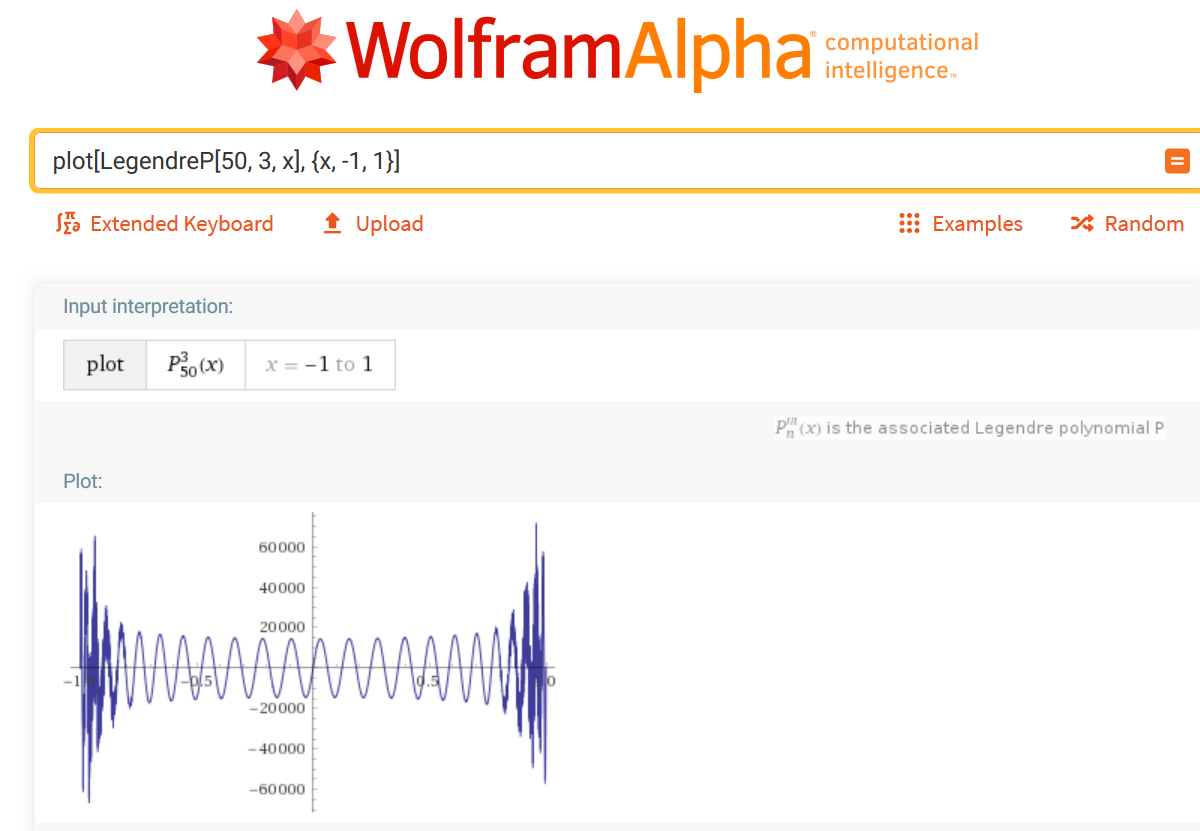
\includegraphics[width=0.9\linewidth]{papers/legendre/plots/wolframalpha}
\caption{Von Wolram Alpha \cite{legendre:wolfram-alpha} generierter Graph des zugeordneten Legendrepolynoms mit Grad 50 und Ordnung 3. Deutliche numerische Instabilitäten nahe den Randbereichen.}
\label{legendre:fig:wolframalpha}
\end{figure}
